% -----------------------------*- LaTeX -*------------------------------
\documentclass[12pt]{report}
\usepackage{%
	amsfonts,%
	amsmath,%	
	amssymb,%
	amsthm,%
	algorithm,%
%	babel,%
	bbm,%
	etex,%
	%biblatex,%
	caption,%
	centernot,%
	color,%
	dsfont,%
	enumerate,%
	epsfig,%
	epstopdf,%
	geometry,%
	graphicx,%
	hyperref,%
	latexsym,%
	mathtools,%
	multicol,%
	pgf,%
	pgfplots,%
	pgfplotstable,%
	pgfpages,%
	proof,%
	psfrag,%
	subfigure,%	
	tikz,%
	ulem,%
	url%
}	
\usepackage[noend]{algpseudocode}
\usepackage[mathscr]{eucal}
\usepgflibrary{shapes}
\usetikzlibrary{%
  	arrows,%
	backgrounds,%
	chains,%
	decorations.pathmorphing,% /pgf/decoration/random steps | erste Graphik
	decorations.text,%
	matrix,%
  	positioning,% wg. " of "
  	fit,%
	patterns,%
  	petri,%
	plotmarks,%
  	scopes,%
	shadows,%
  	shapes.misc,% wg. rounded rectangle
  	shapes.arrows,%
	shapes.callouts,%
  	shapes%
}

\theoremstyle{plain}
\newtheorem{thm}{Theorem}[section]
\newtheorem{lem}[thm]{Lemma}
\newtheorem{prop}[thm]{Proposition}
\newtheorem{cor}[thm]{Corollary}

\theoremstyle{definition}
\newtheorem{defn}[thm]{Definition}
\newtheorem{conj}[thm]{Conjecture}
\newtheorem{exmp}[thm]{Example}
\newtheorem{assum}[thm]{Assumption}
\newtheorem{axiom}[thm]{Axiom}

\theoremstyle{remark}
\newtheorem{rem}{Remark}
\newtheorem{note}{Note}
\newtheorem{fact}{Fact}

\newcommand{\norm}[1]{\left\lVert#1\right\rVert}
\newcommand{\indep}{\!\perp\!\!\!\perp}
\DeclarePairedDelimiter\abs{\lvert}{\rvert}%
\newcommand\numberthis{\addtocounter{equation}{1}\tag{\theequation}}
\newcommand{\tr}{\operatorname{tr}}
\newcommand{\R}{\mathbb{R}}
\newcommand{\N}{\mathbb{N}}
\newcommand{\E}{\mathbb{E}}
\newcommand{\Z}{\mathbb{Z}}
\newcommand{\B}{\mathscr{B}}
\newcommand{\C}{\mathcal{C}}
\newcommand{\T}{\mathscr{T}}
\newcommand{\F}{\mathcal{F}}
\newcommand{\G}{\mathcal{G}}
%\newcommand{\ba}{\begin{align*}}
%\newcommand{\ea}{\end{align*}}
\newcommand{\expect}[1]{\mathbb{E}\left[{#1}\right]}
\newcommand{\prob}[1]{\mathbb{P}\left[{#1}\right]}
\newcommand{\probo}[1]{\mathbb{P}_0\left[{#1}\right]}
\newcommand{\probi}[1]{\mathbb{P}_1\left[{#1}\right]}
\newcommand{\given}{\; \big\vert \;} 
\newcommand{\bydef}{:=}
\newcommand{\indic}[1]{\mathbbm{1}\{#1\}}
\DeclareMathOperator*{\argmax}{arg\,max}
\renewcommand{\qedsymbol}{$\blacksquare$}
\makeatletter
\def\BState{\State\hskip-\ALG@thistlm}
\makeatother

\makeatletter
\def\th@plain{%
  \thm@notefont{}% same as heading font
  \itshape % body font
}
\def\th@definition{%
  \thm@notefont{}% same as heading font
  \normalfont % body font
}
\makeatother
\date{}
\usepackage{graphicx}
\usepackage{times}
\newcommand\independent{\protect\mathpalette{\protect\independenT}{\perp}}
\def\independenT#1#2{\mathrel{\rlap{$#1#2$}\mkern2mu{#1#2}}}
\usepackage{mathtools}
\usepackage{times}
\usepackage{amsmath}
\usepackage{graphics}
\graphicspath{ {C:/Users/hp/Desktop/Detandest_scribing/Estimation-Detection-master/images/} }
\usepackage{scribe_e1244}
%\newtheorem{defn}[thm]{Definition}
%\newtheorem{lem}{Lemma}[thm]
%\newenvironment{definition}[1][Definition]{\begin{trivlist}
%\item[\hskip \labelsep {\bfseries #1}]}{\end{trivlist}}
\begin{document}
	\lecturer{Aditya Gopalan}		
	\scribe{Kanduru Venkata Sesha Sai Sushanth\&Juganta Kishore Saikia}	% required, put your name here
	\lecturenumber{12}			% required, must be a number
	\lecturedate{February 14}		% required, omit year
	\maketitle
	
	% title of the lecture
	\begin{center}
		{\Large \bf  PURELY STOCHASTIC SIGNALS }
	\end{center}
	Recap: Signal Detection in noise
	
	    - Deterministic signals

	    - Partly stochastic signals(Signals with Random parameters)
	
	    - Purely Stochastic signals(This Lecture)
	
	\section{Detection of Stochastic Signals in Noise}
	The basic problem that we are dealing is the following hypothesis testing problem:
	\begin{center}
		$H_0 :  \underline{Y}  =   \underline{N}$
	\end{center}
	\begin{center}
		$H_1 : \underline{Y} =  \underline{S}+ \underline{N}$
	\end{center}
	
	\noindent Where $\underline{N}$ is iid noise with zero mean and $\underline{S}$ is the purely stochastic signal with covariance matrix $\Sigma_s$ that we are dealing with. And also $\underline{S}$ and $\underline{N}$ are independent. 
	
	\begin{center}
		$\underline{N}\sim \mathcal{N}(\underline{0},\sigma^2I )$ , $\underline{S}\sim(\underline{0},\Sigma_s )$ and $\underline{S} \independent \underline{N}$ \par
	\end{center}
	\noindent Motivation: Signals in turbulent/highly random environments. e.g. radio astronomy,sonar,underwater signaling etc. In a more general scenario we have :
	
	\begin{center}
		$ H_0 :  \underline{Y}\sim  \mathcal{N}(\mu_0,\Sigma_0 )$
		\linebreak
		vs 
		\linebreak
		$ H_1 : \underline{Y}\sim \mathcal{N}(\mu_1,\Sigma_1 )$
	\end{center}
	
	\noindent The Log likelihood ratio of the observation $\underline{y}\epsilon R^n$ is\\
	\begin{center}
		$log(L(\underline{y}))=log(\frac{P_1(\underline{y})}{P_0(\underline{y})})$
	\end{center}
	
	\begin{center}
		$log(L(\underline{y}))=log(\frac{\frac{1}{(2\pi)^{0.5}|\Sigma_1|^0.5}exp(\frac{-(\underline{y}-\underline{u}_1)^T\Sigma_1^{-1}(\underline{y}-\underline{u}_1)}{2})}{\frac{1}{(2\pi)^{0.5}|\Sigma_0|^0.5}exp(\frac{-(\underline{y}-\underline{u}_0)^T\Sigma_0^{-1}(\underline{y}-\underline{u}_0)}{2})})$
	\end{center}
	
	
	\begin{center}
		$log(L(\underline{y}))=(1/2) \underline{y}^T(\Sigma_0^{-1}-\Sigma_1^{-1}) \underline{y}+\underline{y}^T(-\Sigma_0^{-1}\mu_0+\Sigma_1^{-1}\mu_1)+C$\\
	\end{center}
	
	\noindent Note : C is a constant that does not depend on $\underline{y}$\\
	
	\noindent Case-(i): When $\Sigma_0=\Sigma_1$.
	\noindent Here the optimum detector is Linear detector and it is given by thresholding a Linear function of $\underline{y}$,ie.
	\begin{center}
		$ y^T\Sigma_0^{-1}(\mu_1-\mu_0)\gtreqqless $.....
	\end{center}
	\noindent Case-(ii):  When $\mu_0=\mu_1=0$\\
	In this we get  a quadratic detector which is of the following form
	\begin{center}        
		. $y^T(\Sigma_0^{-1}-\Sigma_1^{-1})y\gtreqqless $.....
	\end{center}
	Since $\underline{y}^T\underline{y}$ gives energy, in general we can say that it is a " Energy Detector".  More Specifically we can say that it is a " Weighted Energy Detector" . For the following case of hypothesis \\
	\begin{center}
		$H_0 :  \underline{Y}  =   \underline{N}$
		\linebreak
		vs 
		\linebreak
		$H_1 : \underline{Y} =  \underline{S}+ \underline{N}$
	\end{center}
	The optimum detector is : ( For the above case $ \Sigma_0=\sigma^2I,\Sigma_1=\sigma^2I+\Sigma_s$)\\
	
	\begin{equation}
	\delta_0 (\underline{y}) =  
	\begin{cases}
	1, &\underline{y}^TQ\underline{y}>\tau^1   \\
	\gamma,&\underline{y}^TQ\underline{y}=\tau^1 \\
	0,&\underline{y}^TQ\underline{y}<\tau^1
    \end{cases} 
	\end{equation}
	
	Where,\linebreak
	\begin{center}
	 $ Q=\frac{1}{\sigma^2}I - (\sigma^2I+\Sigma_s)^{-1}$\\
	 
	
     $Q=(I+\frac{1}{\sigma^2}\Sigma_s-I) (\sigma^2I+\Sigma_s)^{-1}$\\
     
	
 $Q=(\sigma^2\Sigma_s) (\sigma^2I+\Sigma_s)^{-1}$\\
	\end{center}
 $\underline{y}^TQ\underline{y}\gtreqqless \ldots$ is called a "Weighted energy detector" or a "Radiometer".\\
	
	\section { Performance analysis of a quadratic detector:}
	
	\noindent  Here want to find :        $ P_j[ \underline{Y}^TQ\underline{Y}>\tau^1]$ where j  $\epsilon$ \{0,1\} \\
	
	\noindent So we have to Decompose $ \Sigma_s$ using Singular Value Decomposition(SVD) \\
	
	\begin{center}
 $$\Sigma_s=\sum_{k=1}^{n} \lambda_k\underline{v}_k\underline{v}^T $$
	\end{center}
	\noindent where $\{\underline{v}_1,\underline{v}_2,\ldots,\underline{v}_n$\} are " Ortho Normal" and also we can express I as  $I= \sum_{k=1}^{n}\underline{v}_k\underline{v}^T$\\
	
	\noindent Using the expressions for $ \Sigma_s$ and I as given above, we can write the following\\
	\begin{center}
		$ (\sigma^2I+\Sigma_s)^{-1}= \sum_{k=1}^{n}( \lambda_k+\sigma^2)^{-1}\underline{v}_k\underline{v}^T $\\
	\end{center}
	\noindent and hence we can write the following expression \\
	\begin{center}
		\ $ (\sigma^2\Sigma_s) (\sigma^2I+\Sigma_s)^{-1}=\sum_{k=1}^{n}(\frac{\lambda_k}{(\lambda_k+\sigma^2)\sigma^2})\underline{v}_k\underline{v}^T$\\
	\end{center}
	\noindent So we finally obtain the following expression with the help of SVD \\
	\begin{center}
		$\underline{y}^TQ\underline{y}=\sum_{k=1}^{n} y_k^{2}$\\
	\end{center}
	
	\noindent where\\
	\begin{center}
		$y_k=(\sqrt(\frac{\lambda_k}{(\lambda_k+\sigma^2)\sigma^2}))\underline{y}^T\underline{v}_k$\\
	\end{center}
	
	\noindent Exercise : Suppose if Y is multivariate then show that  \\
	\begin{center}
	\noindent $ \bar{Y}_k=(\sqrt(\frac{\lambda_k}{(\lambda_k+\sigma^2)\sigma^2}))\underline{Y}^T\underline{v}_k$
	\end{center}
  Where $\bar{Y}_k $  for $ k=1,\ldots,n$ are independent, Guassian random variables with mean zero \\
	
	\noindent Let $\sigma_{jk}^{2}=var(\bar{Y}_k|H_j)$ for j=0,1 and k=1,$\ldots,n$ 
	
	\begin{equation}
     \sigma_{jk}^{2} =
	\begin{cases}
	\frac{\lambda_k}{(\lambda_k+\sigma^2)} ,& j=0\\
	\frac{\lambda_k}{\sigma^2},& j=1\\
	\end{cases}
	\end{equation}
	
\noindent The pdfs of $ T_k=\bar{Y}_k^{2}$ under $ H_j$ is :\\
\begin{equation}
	P_{T_k}(t|H_j)=
	\begin{cases}
	\frac{1}{(\sqrt{2\pi t}\sigma_{jk}}e^{\frac{-t}{2\sigma_{jk}^{2}}},& t>=0\\
	0,& t<0\\
	\end{cases}
\end{equation}	
\noindent This is a gamma Density with parameters 	$ \frac{1}{2}, \frac{-1}{2\sigma_{jk}^{2}}$\\

\noindent For a Gamma Density with parameters a and b i.e GAMMA(a,b), the pdf is $\alpha$ $x^{a-1}e^{-bx}$\\
	
\noindent	Hence the pdf of $ T=  \sum_{k=1}^{n}T_k$       where $T_k=\underline{Y}^TQ\underline{Y}$ is given as \\
\begin{center}	
\noindent	$P_T=P_{T_1}\ast P_{T_2}\ast \ldots P_{T_n}$      where $\ast$ denotes convolution\\
\end{center}
\noindent	$P_T=\mathcal{F}^{-1}[\prod_{k=1}^{n}\phi_{T_k}]$ , where $\phi_{T_k}$ is the charecteristic function of $T_k$ and is given as :\\
\begin{center}
\noindent  	$\phi_{T_k}(u)=\mathcal{E}[e^{iuT_k}]$ where $f_X(x)=\frac{1}{2}\int_{-\infty}^{\infty}\phi_X(t)e^{-itx}dt$\\

\end{center}
\begin{center}
\noindent$P_T(t|H_j)=\frac{1}{2\pi}\int_{-\infty}^{\infty}e^{-itu}\prod_{k=1}^{n}\phi_{T_k}(u)du$\\
\end{center}	
	
	
\noindent	For the case of Gamma Distribution, the charecteristic function is given by $\phi_{T_k}(u)=[1-2iu\sigma_jk^{2}]^{-1}$\\
	
\noindent	Generally $P_T(t|H_j)$ is intractable, but it is possible to find when $\sigma_{j1}=\sigma_{j2}=\ldots=\sigma_{jk}=\sigma_j$ where j=0,1\\
	
\noindent In this Special case,\\
\begin{center}	
\noindent	$P_T(t|H_j)=GAMMA(\frac{n}{2},\frac{-1}{2\sigma_j^{2}})=\Gamma(\frac{n}{2},\frac{-1}{2\sigma_j^{2}})$\\
\end{center}
\begin{center}	
\noindent	$\sigma_{j1}=\sigma_{j2}=\ldots=\sigma_{jk}=\sigma_j$ if and only if $\lambda_1=\lambda_2=\ldots=\lambda_n=\sigma_n^{2}$\\
\end{center}
\begin{center}
\noindent	$\Sigma_s=\sigma_s^{2}I$ i.e $\underline{S}\sim\mathcal{N}(\underline{0},\sigma_s^{2}I)$\\
\end{center}	
\noindent	Hence,
\begin{center}
 $\mathcal{P}_j[\underline{Y}^TQ\underline{Y}>\tau^1]=1-\Gamma(\frac{n}{2},\frac{\tau^1}{2\sigma_j^{2}})$\\
\end{center}
\noindent	where $\Gamma(\frac{n}{2},\frac{\tau^1}{2\sigma_j^{2}})$ is the CDF of $\underline{Y}^TQ\underline{Y}$ at $\tau^1$. This is an "Incomplete Gamma Function"\\
	
\noindent eg: For False alarm probability $\alpha$,\\
\begin{center}		
\noindent	$\tau^1=2\sigma_0^{2}\Gamma^{-1}(\frac{n}{2},1-\alpha)$\\
\end{center}	
\noindent	Correspondingly,\\
	\begin{center}
\noindent	$P_D=1-\Gamma(\frac{n}{2},\frac{\sigma_0^{2}}{\sigma_1^{2}}\Gamma^{-1}(\frac{n}{2},1-\alpha))$\\
\end{center}
\noindent	Note: \\
	
\noindent	Performance of this detector is a function of \\
	
\noindent	1) n  (i.e size of the vector)  \\
\noindent2)$\frac{\sigma_0^{2}}{\sigma_1^{2}}=\frac{\frac{\sigma_s^{2}}{\sigma_s^{2}+\sigma^2}}{\frac{\sigma_s^{2}}{\sigma^2}}=\frac{1}{1+\frac{\sigma_s^{2}}{\sigma^2}}$\\
	
\noindent \section{Detector Structure} $\underline{y}^TQ\underline{y}\gtreqqless\ldots$
\noindent  where  Q=$(\sigma^2\Sigma_s)(\sigma^2I+\Sigma_s)^{-1}$\\

\noindent (i)Decorrelator-Energy Detector:\\
\noindent The block diagram of this type of detector is as shown in the Figure \ref{fig:energydetector}.Where $ \{v_1,v_2,v_3..........v_n\} $ is the orthonormal basis w.r.t $ \Sigma_s $\\
		\begin{figure}%[h]
		\centering
		\scalebox{0.65}
		{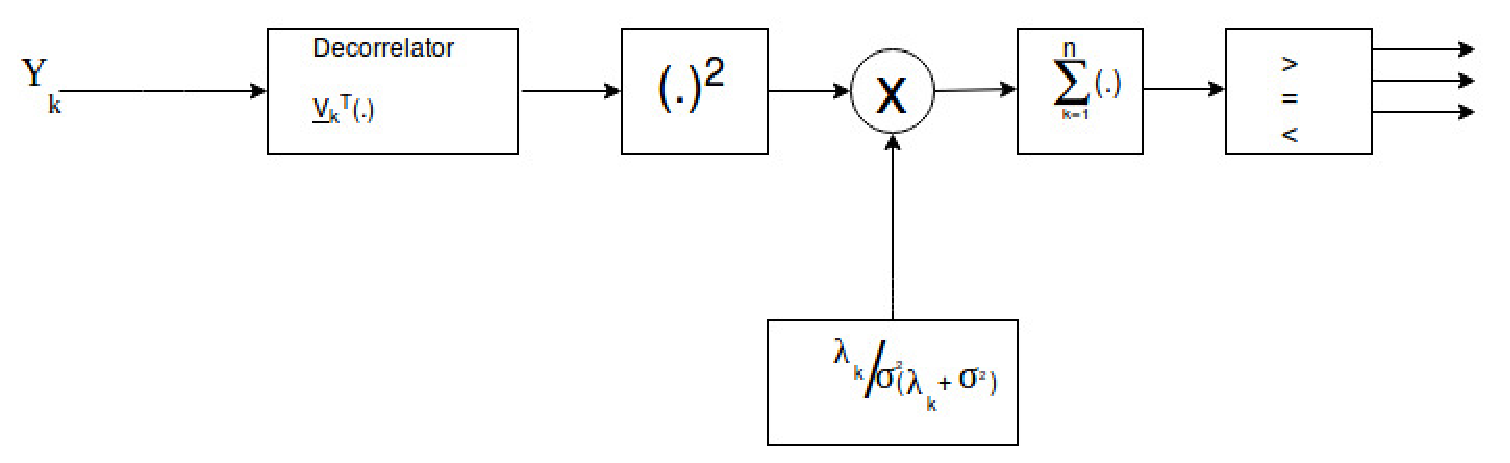
\includegraphics{EnergyDetector}}\\
			\caption{Decorrelator-Energy Detector}
		\label{fig:energydetector}
	\end{figure}

\noindent (ii)Estimator-Correlator Detector:\\
\noindent The block diagram of this type of detector is as shown in the Figure\ref{fig:EstCorrelator}
	
	\begin{figure}%[h]
		\centering
		\scalebox{0.60}
		{\includegraphics{Estimator_Correlator}}\\
			\caption{Estimator Correlator}
		\label{fig:EstCorrelator}
		
		
		
	\end{figure}



	
\end{document}